\documentclass[lettersize,journal]{IEEEtran}

\usepackage{amsmath,amsfonts,amssymb}
\usepackage{array}
\usepackage{stfloats}
\usepackage{url}
\usepackage{graphicx}
\usepackage{cite}
\hyphenation{op-tical net-works semi-conduc-tor IEEE-Xplore}
\def\BibTeX{{\rm B\kern-.05em{\sc i\kern-.025em b}\kern-.08em
    T\kern-.1667em\lower.7ex\hbox{E}\kern-.125emX}}

\urlstyle{same}

% Float spacing: IEEEtran defaults leave generous gaps around floats.
% Tightened to recover vertical space without altering figure content.
\setlength{\textfloatsep}{4pt plus 1pt minus 1pt}
\setlength{\floatsep}{6pt plus 2pt minus 2pt}
\setlength{\intextsep}{6pt plus 2pt minus 2pt}
\setlength{\dbltextfloatsep}{4pt plus 1pt minus 1pt}
\setlength{\dblfloatsep}{6pt plus 2pt minus 2pt}
\setlength{\abovecaptionskip}{3pt}
% Float packing: IEEEtran's defaults reserve a large fraction of each
% column for text, which strands whitespace on figure-heavy pages.
% Raising the float fractions lets LaTeX fill those pages properly.
\renewcommand{\topfraction}{0.95}
\renewcommand{\bottomfraction}{0.95}
\renewcommand{\textfraction}{0.05}
\renewcommand{\floatpagefraction}{0.85}
\renewcommand{\dbltopfraction}{0.95}
\renewcommand{\dblfloatpagefraction}{0.85}
\setlength{\belowcaptionskip}{0pt}

\begin{document}

\title{Second-Order Cooperative Field Estimation and Tracking of Coherent Flow Structures Using Multirobot Systems}

\author{Christopher Waight and Christopher A. Kitts,~\IEEEmembership{Senior Member,~IEEE}
\thanks{C. Waight is a PhD Candidate in the Robotic Systems Laboratory, Department of Mechanical Engineering, Santa Clara University, Santa Clara, CA 95053 USA (e-mail: cwaight@scu.edu)}
\thanks{C. A. Kitts is Professor and Director of the Robotic Systems Laboratory, Department of Mechanical Engineering, Santa Clara University, Santa Clara, CA 95053 USA (e-mail: ckitts@scu.edu)}
}
\markboth{IEEE Systems Journal}%
{Waight and Kitts: Second-Order Cooperative Field Estimation for Multirobot Tracking of Coherent Flow Structures}

\maketitle

\begin{abstract}
Adaptive navigation is the process of modifying the motion of a robot's or a system of robots' based on 
real-time measurements taken from the environment being traversed. This paper 
develops an Adaptive Navigation strategy to navigate two short term flow transport boundaries; the strain-dominated
curves across which water masses separate and the curves along which floating material collects.
Existing robotic trackers of these structures prestraddle it before tracking begins and either commits to the structure's
identity or accumulate an estimate over a finite integration horizon to determine the type.
We show that a computed second-order polynomial fit of the local flow can be recovered using synchronized measurements from six robots.
This quadratic surrogate model can be used as a foundation to calculate two derived fields which map the vector field to a scalar invariant field:
The Jacobian determinant field and the smaller rate of strain eigenvalue field.
We develop two adaptive navigation primitives to steer on each of these derived fields along the transport boundaries. Each tracker locates the nearest separating boundary
and navigates to and along it from instantaneous measurements, with no integration horizon or prestraddling requirements.
Monte Carlo analysis shows that the determinant tracker withstands more measurement noise than the rate of strain tracker from every tested starting position.
However, the rate of strain tracker is objective in nature, and holds the the desired trajectory when the observer is rotating while the Jacobian determinant tracker fails.
On Santa Barbara Channel radar currents, both primitives follow the dominant transport corridor from coast to coast.

\end{abstract}

\begin{IEEEkeywords}
Mobile Robots, Multirobot Systems, Adaptive Navigation, Coherent
Structures, Rate of Strain, Objectivity, Cooperative Estimation,
Cluster Space Control
\end{IEEEkeywords}

\section{Introduction}


\IEEEPARstart{M}{ultirobot} systems (MRS) offer redundancy, increased
throughput, and cooperative capabilities a single robot cannot produce,
and have proven operational success  across land, sea, air, and space \cite{1,2}.
Furthermore, and MRS can tolerate individual robot failures and adapt their formation based on mission objectives. \cite{3,4,5}.

In adaptive
navigation (AN), a vehicle or group of vehicles modifies its velocity and desired trajectory in real time
as it creates a local map from measurements taken while moving \cite{3}. A single vehicle must translate to sense a
gradient, which costs time and memory and misleads in a time-varying field,
whereas an MRS can sample multiple locations simultaneously, enabling faster reaction times and better performance in non-static fields.


AN in scalar fields is well. Each
robot contributes one scalar measurement to a contol policy that controls the robots to reach or
follow a feature. For example, specific formations are held so that differential measurements across different robots
recover the gradient and curvature needed for specific control policies
 \cite{5,6}. 
 \"{O}gren, Fiorelli, and Leonard
established cooperative gradient climbing with a formation of mobile
sensors using plane fitting \cite{6}. Bri\~{n}\'{o}n-Arranz, Renzaglia, and Schenato
extended the fitting process to recover the Hessian by exploiting the gradients and curvature calculated from five robots on a ring plus one at the
center \cite{5}. Kitts, McDonald, and
Neumann developed primitives for extrema finding, contour following,
ridge/trench following, and saddle point station keeping \cite{3}, and
verified ridge, trench, saddle, and front tracking experimentally on an
indoor testbed \cite{4,7}.

%% Going through this document again

Some physical environments are better represented as vector fields, which can model certain features that have no scalar field equivalents. 
Critical points, such as sinks, sources, and vortices, can model convergence zones \cite{8} and subsurface leaks \cite{9}. In \cite{10} a three-robot cluster
estimated the location and type of a nearby critical point  from a linear fit of
simultaneous local velocity measurements and used this estimate to adaptively navigate towards and orbit it. 

Vector fields also have well defined curves that are useful for modelling naturally occuring phenomenon. 
For example, dynamic ocean flows contain naturally occurring boundaries known as coherent structures that influence where floating materials like debris and larvae will accumulates or separate \cite{11,12}.
Coherent structures are typically identified through one of two primary methods.
The first relies on Lagrangian coherent structures (LCS) \cite{16}, typically computed as ridges in the finite-time Lyapunov exponent field \cite{17}. 
The second method uses instantaneous Eulerian criteria, such as the Okubo-Weiss parameter, to partition flows based solely on the local velocity gradient \cite{8,22}.
This instantaneous approach has been generalized to three dimensions \cite{23}, refined to second order \cite{24}, and applied at scale in mesoscale eddy censuses \cite{25}. 
The tradeoffs between using a Lagrangian or an Eulerian approach is a matter of ongoing research \cite{18,19,20,21}.


Mapping these curves allows teams to deploy resources in highly targeted search areas \cite{12,13,14,15}. 
Traditionally, Without adaptive navigation, a large scale team must sample a much larger basin to determine where these structures lie using offline reconstruction.
Adaptive Navigation, however, allows for quick localized mapping of this curve with a small team. 


Recent work has begun applying AN techniques with MRS's to navigate along coherent structures.
 Michini et al. travel along a presumed stable or
unstable manifold with three robots using only local velocity
measurements \cite{26}, an approach inspired by the PIM triple
procedure \cite{27}  \cite{28}.  The saddle point is not discussed by neither the
controller nor its analysis, and that work reports veering away from
the structure near a saddle in flow-tank experiments.
 Kularatne and Hsieh confirm the boundary of the attracting surface by computing the local FTLE field on board at the cost of a nonzero integration horizon \cite{29}.
In these studies, the robotic teams pre-straddle the structure, and do not acquire a structure if they aren't.


This paper uses an eularian specification of the flow field, and shows that a second-order polynomial fit of the local flow can be used to
acquire and track such a structure from instantaneous measurements. 
The contributions are
\begin{itemize}
\item a cooperative estimator that recovers the local quadratic model of
a two-component field from one synchronized set of measurements across six robots that fails only when the robots
lie on a common conic;
\item two surrogates fields transformed by that fit: the
determinant field $D$ and the smaller strain eigenvalue field
$s_1$ ;

\item two AN primitives, the $D$ tracker and the $s_1$ tracker, that
navigate to the structure and ride along it without pre-straddling;
\item a compairson of the trackers showing the $D$ tracker tolerates more
measurement noise while the $s_1$ tracker, being objective, holds its
path under a rotating observer, which matters when the measured flow
carries the observer's own rotation.
\end{itemize}

Both primitives run on a simulated double gyre and on measured Santa
Barbara Channel radar currents.

\section{Second-Order Field Estimation}

\subsection{Local Vector Field Polynomials}

A planar vector field assigns a velocity $\mathbf{v}(\mathbf{p}) =
(u(\mathbf{p}), v(\mathbf{p}))$ to each position in space $\mathbf{p} = (x, y)$.
The critical point estimator of \cite{10} fits a plane to each
component of the vector field and solves for the point where $\mathbf{v} = \mathbf{0}$. 

In this work, we extend the linear approximation to the second-order Taylor expansion about the
centroid, $\mathbf{p}_c$. Coordinates are measured
from the centroid throughout this section, so $\mathbf{p}_c = \mathbf{0}$.
\begin{align}
    u(\mathbf{p}) &= a_1 + a_2 x + a_3 y
        \nonumber \\
        &\quad + a_4 xy + \tfrac{1}{2} a_5 x^2 + \tfrac{1}{2} a_6 y^2
        + \mathcal{O}(\|\mathbf{p}\|^3),
        \label{eq:quad_model_u} \\
    v(\mathbf{p}) &= b_1 + b_2 x + b_3 y
        \nonumber \\
        &\quad + b_4 xy + \tfrac{1}{2} b_5 x^2 + \tfrac{1}{2} b_6 y^2
        + \mathcal{O}(\|\mathbf{p}\|^3),
        \label{eq:quad_model_v}
\end{align}
where $\mathcal{O}(\|\mathbf{p}\|^3)$ is the truncation error.
The twelve coefficients of this quadratic model are constants and each is a derivative of the field at
the centroid. The one-half factors cancel the factor of 2 during differentiation.
This gives $a_1 = u(\mathbf{p}_c)$, $a_2 = \partial u/\partial
x|_{\mathbf{p}_c}$, $a_3 = \partial u/\partial y|_{\mathbf{p}_c}$,
$a_4 = \partial^2 u/\partial x \partial
y|_{\mathbf{p}_c}$, $a_5 = \partial^2 u/\partial x^2|_{\mathbf{p}_c}$,
$a_6 = \partial^2 u/\partial y^2|_{\mathbf{p}_c}$,
and likewise for $b_1, \ldots, b_6$ with $v$ in place of $u$.

To estimate these coefficients with robot positions $\mathbf{p}_i = (x_i,
y_i)$, we define the quadratic basis vector
\begin{equation}
    \boldsymbol{\phi}(\mathbf{p}) =
    \bigl[\,1, \; x, \; y, \; xy, \;
    \tfrac{1}{2}x^2, \; \tfrac{1}{2}y^2\,\bigr]^\top,
\end{equation}
whose entries are the terms of
(\ref{eq:quad_model_u})--(\ref{eq:quad_model_v}) in order, so
the recovered coefficients, which we mark with a hat, estimate the Taylor derivatives directly with
no rescaling. Stacking the six basis vectors row-wise gives
the $6 \times 6$ formation matrix $\boldsymbol{\Phi}$, and the coefficient
estimates $\hat{\boldsymbol{\theta}}_u = [\hat{a}_1, \ldots,
\hat{a}_6]^\top$ and $\hat{\boldsymbol{\theta}}_v = [\hat{b}_1, \ldots,
\hat{b}_6]^\top$ solve
\begin{equation}
    \boldsymbol{\Phi}\,\hat{\boldsymbol{\theta}}_u = \mathbf{m}_u, \qquad
    \boldsymbol{\Phi}\,\hat{\boldsymbol{\theta}}_v = \mathbf{m}_v,
    \label{eq:solve}
\end{equation}
where $\mathbf{m}_u = [u_1, \ldots, u_6]^\top$ and
$\mathbf{m}_v = [v_1, \ldots, v_6]^\top$ collect the measurements $u_i$ and $v_i$, the components of the velocity
sampled by robot $i$. 

\subsection{Minimality}
\label{sec:minimality}

Six robots is the minimum for recovery of the unconstrained local
quadratic model of a two-component planar field from one synchronized set of measurements. Each robot contributes one equation per component to
(\ref{eq:solve}), and each system has six unknowns, so fewer than six
robots leave the solution set a positive-dimensional affine subspace.

Six robots suffice provided $\boldsymbol{\Phi}$ is nonsingular. With
more than six, $\boldsymbol{\Phi}$ has more rows than columns, the fit
becomes least squares, and the condition becomes full column rank.
Either condition fails exactly when the robots lie on a common conic.
For example, a standard ring formation is degenerate at any size, since
the ring itself is the conic. A fit from more than six robots also
leaves a residual, which carries the measurement noise and the
truncation error.

With five equations or fewer, a method either returns a family of solutions or imposes a structural prior, such as assuming
divergence-free flow by imposing $\nabla\cdot\mathbf{v} = 0$. We do not impose any priors on the field, as horizontal surface
currents are not divergence free, so imposing
$\nabla\cdot\mathbf{v} = 0$ would bias every recovered coefficient.

For this study, we chose the pentagon-plus-center formation and use it
throughout. It is the smallest uniform ring plus center on which \cite{5}
recovers a scalar Hessian exactly for quadratic signals, independent of
the formation's orientation. The same symmetry makes the noise gains of
the fit here independent of formation heading.


\subsection{Estimator Sensitivity}
\label{sec:sensitivity}

The accuracy of the estimator is affected by the formation of the
robots, the noise on each robot's measurements, and the error in each
robot's position.

\subsubsection{Formation}
The rank of the formation matrix $\boldsymbol{\Phi}$ determines whether
a unique fit exists, and its condition number $\kappa(\boldsymbol{\Phi})$
indicates how much the fit amplifies noise. Condition numbers are
reported on the radius-normalized $\boldsymbol{\Phi}$, with each column
of order $q$ divided by $\rho^{\,q}$, where $\rho$ is the formation radius. Without this normalization, the
quadratic columns shrink as $\rho^{2}$ and a healthy formation would
appear degenerate. The normalized matrix depends only on the formation's
shape, and the pentagon-plus-center formation gives
$\kappa(\boldsymbol{\Phi}) = 8.26$ at every radius. The size of the formation does not change
$\kappa(\boldsymbol{\Phi})$, but it does change how much noise reaches
each coefficient. A coefficient of order $q$ is recovered from
differences in readings across the footprint divided by $\rho^{\,q}$, so
the same measurement noise produces a coefficient error that scales as
$\rho^{-q}$. A larger formation therefore suppresses noise most in the
second-order terms, but it also increases the truncation error
$\mathcal{O}(\|\mathbf{p}\|^3)$, since the ring robots sit at
$\|\mathbf{p}\| = \rho$. The condition number grows as the robots
drift toward a common conic. For example, moving the center robot out
to $0.99\rho$ places all six robots within $0.6\%$ of a common circle
and raises $\kappa(\boldsymbol{\Phi})$ to $564$. The fit degrades
continuously on the way to the degeneracy of
Section~\ref{sec:minimality}, with no threshold at which it fails.

\subsubsection{Measurement Noise}
Each robot carries its own sensor, so the measurement noise of one robot
is independent of the others. Furthermore, the estimator uses only
instantaneous readings, so each cycle's fit sees only that cycle's
noise. The noise is modeled as additive on each reading,
\begin{equation}
    u_i^m = u(\mathbf{p}_i) + \eta_i^u, \qquad
    v_i^m = v(\mathbf{p}_i) + \eta_i^v,
    \label{eq:meas_noise}
\end{equation}
with $\eta \sim \mathcal{N}(0, \sigma_{uv}^2)$. The fit is linear in the
measurements, so the noise reaches the coefficients as
$\boldsymbol{\Phi}^{-1}\boldsymbol{\eta}^u$ and
$\boldsymbol{\Phi}^{-1}\boldsymbol{\eta}^v$, where $\boldsymbol{\eta}^u$
and $\boldsymbol{\eta}^v$ stack the noise of the six robots. Both are
zero-mean, so measurement noise adds no bias to the coefficient estimates.

\subsubsection{Position Noise}
A robot with position error
$\boldsymbol{\xi}_i \sim \mathcal{N}(\mathbf{0}, \sigma_p^2\mathbf{I})$
samples the field at $\mathbf{p}_i + \boldsymbol{\xi}_i$, but the fit is
built from its nominal position $\mathbf{p}_i$. The formation matrix is
therefore wrong by $\Delta\boldsymbol{\Phi}$, whose row $i$ is
$\boldsymbol{\phi}(\mathbf{p}_i + \boldsymbol{\xi}_i)^{\top} -
\boldsymbol{\phi}(\mathbf{p}_i)^{\top}$. Under the quadratic model the
measurements are
$\mathbf{m}_u = (\boldsymbol{\Phi} + \Delta\boldsymbol{\Phi})
\boldsymbol{\theta}_u$, and the fit returns
\begin{equation}
    \hat{\boldsymbol{\theta}}_u = \boldsymbol{\theta}_u
        + \boldsymbol{\Phi}^{-1}\Delta\boldsymbol{\Phi}\,
          \boldsymbol{\theta}_u ,
    \label{eq:pos_noise}
\end{equation}
and likewise for $\hat{\boldsymbol{\theta}}_v$. To first order, entry
$i$ of $\Delta\boldsymbol{\Phi}\,\boldsymbol{\theta}_u$ is
$\nabla u \cdot \boldsymbol{\xi}_i$, the change in $u$ across the
displacement. This error vanishes in uniform flow and grows with the
local gradient, so unlike measurement noise it depends on the field.
Its variance is $\lVert\nabla u\rVert^2\sigma_p^2$ for $u$ and
$\lVert\nabla v\rVert^2\sigma_p^2$ for $v$, and the two average to
$\tfrac{1}{2}\lVert\mathbf{J}\rVert_F^2\sigma_p^2$, with $\mathbf{J} = \nabla\mathbf{v}$ the velocity gradient tensor and $\lVert\cdot\rVert_F$ the Frobenius norm. Combining both noise
sources gives one effective noise level
\begin{equation}
    \sigma_{\mathrm{eff}}^2 = \sigma_{uv}^2
        + \tfrac{1}{2}\lVert\mathbf{J}\rVert_F^2\,\sigma_p^2 .
    \label{eq:sigma_eff}
\end{equation}



\subsection{Eulerian Surrogates}
\label{sec:surrogates}

Lagrangian methods locate coherent structures by integrating particle
trajectories over a finite time window \cite{16,17}. This paper instead
reads them from the instantaneous geometry of the velocity field, as
Eulerian coherent structures \cite{19}. Two fields computed from the
six-robot fit mark the separatrix. The first is the determinant of the velocity
gradient, and the second is the smaller eigenvalue of its symmetric
part.

\subsubsection{Determinant Field}
The fitted coefficients define the velocity gradient at every point of
the footprint. Differentiating the quadratic model gives a Jacobian whose
entries are affine in position,
\begin{equation}
    \hat{\mathbf{J}}(\mathbf{p}) =
    \begin{bmatrix}
        \hat{a}_2 + \hat{a}_5 x + \hat{a}_4 y &
        \hat{a}_3 + \hat{a}_4 x + \hat{a}_6 y \\
        \hat{b}_2 + \hat{b}_5 x + \hat{b}_4 y &
        \hat{b}_3 + \hat{b}_4 x + \hat{b}_6 y
    \end{bmatrix}.
    \label{eq:Jhat}
\end{equation}
The determinant $\hat{D}(\mathbf{p}) = \det\hat{\mathbf{J}}(\mathbf{p})$
is therefore exactly quadratic over the footprint. Its value, gradient,
and Hessian at the centroid are polynomials in the coefficients. The
value is $\hat{D}_0 = \hat{a}_2\hat{b}_3 - \hat{a}_3\hat{b}_2$, and the
gradient is
\begin{equation}
    \hat{\mathbf{g}}_0 =
    \begin{bmatrix}
        \hat{a}_5\hat{b}_3 + \hat{a}_2\hat{b}_4 - \hat{a}_4\hat{b}_2 - \hat{a}_3\hat{b}_5 \\
        \hat{a}_4\hat{b}_3 + \hat{a}_2\hat{b}_6 - \hat{a}_6\hat{b}_2 - \hat{a}_3\hat{b}_4
    \end{bmatrix}.
    \label{eq:grad_det}
\end{equation}
The Hessian is
\begin{equation}
    \hat{\mathbf{H}}_{D,0} =
    \begin{bmatrix}
        2(\hat{a}_5\hat{b}_4 - \hat{a}_4\hat{b}_5) &
        \hat{a}_5\hat{b}_6 - \hat{a}_6\hat{b}_5 \\
        \hat{a}_5\hat{b}_6 - \hat{a}_6\hat{b}_5 &
        2(\hat{a}_4\hat{b}_6 - \hat{a}_6\hat{b}_4)
    \end{bmatrix},
    \label{eq:hess_det}
\end{equation}
which is constant over the footprint.

For incompressible flow the determinant is a negative multiple of the
Okubo-Weiss parameter \cite{8,22}, so the two carry the same partition of
the flow. Where $D < 0$ the flow is strain-dominated, and where $D > 0$
it is rotation-dominated. In the flows studied here, separatrices run along the trenches of $D$
inside the strain-dominated regions.


\subsubsection{Strain Eigenvalue Field}
The second surrogate comes from the rate-of-strain tensor
$\hat{\mathbf{S}} = \tfrac{1}{2}(\hat{\mathbf{J}} + \hat{\mathbf{J}}^{\top})$,
the symmetric part of the same fitted Jacobian.
At the centroid its mean, deviatoric normal, and shear strain are
$\hat{\mu} = (\hat{a}_2 + \hat{b}_3)/2$,
$\hat{s}_n = (\hat{a}_2 - \hat{b}_3)/2$, and
$\hat{s}_s = (\hat{a}_3 + \hat{b}_2)/2$, and each is affine in position.
The eigenvalues of $\hat{\mathbf{S}}$ are
$\hat{s}_{1,2} = \hat{\mu} \mp \hat{r}$ with
$\hat{r} = \sqrt{\hat{s}_n^2 + \hat{s}_s^2}$. Their eigenvectors
$\mathbf{e}_1$ and $\mathbf{e}_2$ are the compression and stretching
directions. The gradient of the smaller eigenvalue follows by the chain
rule,
\begin{equation}
    \nabla\hat{s}_1 = \nabla\hat{\mu}
        - \frac{\hat{s}_n\nabla\hat{s}_n + \hat{s}_s\nabla\hat{s}_s}{\hat{r}},
    \label{eq:grad_s1}
\end{equation}
where the second-order coefficients give the constant gradients
\begin{equation}
    \begin{aligned}
        \nabla\hat{\mu} &= \tfrac{1}{2}(\hat{a}_5 + \hat{b}_4,\; \hat{a}_4 + \hat{b}_6), \\
        \nabla\hat{s}_n &= \tfrac{1}{2}(\hat{a}_5 - \hat{b}_4,\; \hat{a}_4 - \hat{b}_6), \\
        \nabla\hat{s}_s &= \tfrac{1}{2}(\hat{a}_4 + \hat{b}_5,\; \hat{a}_6 + \hat{b}_4).
    \end{aligned}
    \label{eq:grad_strain}
\end{equation}
The quotient stays bounded as $\hat{r} \to 0$, since $(\hat{s}_n, \hat{s}_s)/\hat{r}$
is a unit vector, but its direction is undefined where $\hat{r} = 0$. Unlike $\hat{D}$, $\hat{s}_1$ has no
usable Hessian. It is an affine function minus the norm of an affine
map, so it is concave over the footprint for every field and formation.

Serra and Haller define objective Eulerian coherent structures (OECS)
from these eigenvalues and eigenvectors \cite{19}. An attracting OECS is a
trench of $s_1$ tangent to $\mathbf{e}_2$, and floating material has been
observed at sea to collect onto such curves \cite{12}. A repelling OECS is a
ridge of $s_2$ tangent to $\mathbf{e}_1$, along which neighboring
material separates. In incompressible flow $s_2 = -s_1$, so repelling
structures are also trenches of $s_1$, and one tracker rides both.

\subsubsection{Relation Between the Fields}
Both fields are read from the same fitted Jacobian, so moving between
them changes nothing in the estimator. Where the vorticity
$\omega = \partial v/\partial x - \partial u/\partial y$ vanishes,
$\mathbf{J}$ equals $\mathbf{S}$ and $D = s_1 s_2$, which is $-s_1^2$ in
incompressible flow. Along such a curve the two fields share their
trenches. Elsewhere the spin $\mathbf{W} = \mathbf{J} - \mathbf{S}$, the
antisymmetric part of $\mathbf{J}$ that carries the vorticity, separates
them. It also separates them across observers. A frame rotating clockwise at rate
$\Omega$, with rotation $\mathbf{Q}$, adds a uniform spin that raises
$\omega$ to $\omega + 2\Omega$. The strain tensor only co-rotates, so
$s_1$ is objective \cite{19}, while the determinant keeps the spin,
\begin{equation}
    D' = D + \Omega\,\omega + \Omega^2 .
    \label{eq:D_not_objective}
\end{equation}
Relatively rotating observers therefore disagree about where the
trenches of $D$ lie. 

\subsection{The Double-Gyre Example}
\label{sec:dg_example}

The double gyre is
a benchmark flow on which both fields mark the material transport structure
exactly, and every
quantity of interest has a closed form. The flow is two counter-rotating gyres in a
closed basin, separated by a separatrix that runs between two saddle points on
the basin walls. We use the steady member of the Shadden
family~\cite{17}, shifted from the canonical domain
$[0,2]\times[0,1]$ to $[-1,1]\times[-0.5,0.5]$ to center it on the origin. The
shift is $x_f = x + 1$, $y_f = y + 0.5$, where $(x_f, y_f)$ are field-frame and
$(x, y)$ world-frame coordinates. Both are non-dimensional throughout the
double-gyre experiments. The field is
\begin{equation}
u = -\pi A \sin(\pi x_f)\cos(\pi y_f), \quad
v = \pi A \cos(\pi x_f)\sin(\pi y_f),
\label{eq:dg_u}
\end{equation}
with $A = 0.1$. The separatrix is the line $x = 0$, the saddle points are
$\mathbf{p}_1^* = (0, -0.5)$ and $\mathbf{p}_2^* = (0, 0.5)$, and the gyre
centers are $(\pm 0.5, 0)$. The field tiles the plane with counter-rotating
gyre cells, and the basin holds one pair of them.

The analytical Jacobian entries are
$u_x = -\pi^2 A \cos\pi x_f \cos\pi y_f = -v_y$ and
$u_y = \pi^2 A \sin\pi x_f \sin\pi y_f = -v_x$, with subscripts denoting
partial derivatives of the true field. The flow is therefore
incompressible, and its determinant and Hessian are
\begin{equation}
\begin{aligned}
D(\mathbf{p}) &= -\tfrac{1}{2}\pi^4 A^2 \left(\cos 2\pi x_f + \cos 2\pi y_f\right),\\
\mathbf{H}_D &= 2\pi^6 A^2
\begin{bmatrix} \cos 2\pi x_f & 0 \\ 0 & \cos 2\pi y_f \end{bmatrix}.
\end{aligned}
\label{eq:det_analytic_main}
\end{equation}
The landscape of $D$ forms a mountain pass over the separatrix
(Fig.~\ref{fig:dg_fields}(b)). Its peaks are the two gyre centers, where
rotation dominates and $D > 0$. Its lowest points are the flow saddles
$\mathbf{p}_1^*$ and $\mathbf{p}_2^*$, joined by a trench along the
separatrix that rises to a crest at the origin, where $D = 0$. The crest
splits the separatrix into an upper and a lower segment. Further trenches
run along the four walls and cross the separatrix at right angles at
$\mathbf{p}_1^*$ and $\mathbf{p}_2^*$, and each other at the four domain
corners, which are also saddle points of the flow.

Across the trench $D$ has constant positive curvature. Along it, each
segment is concave on its inner half and convex on its outer half, so $D$
has a local minimum at each flow saddle.

The $s_1$ landscape has the same trenches (Fig.~\ref{fig:dg_fields}(c)).
The shear strain vanishes identically, since $v_x = -u_y$, so
$\mathbf{S} = \mathrm{diag}(u_x, -u_x)$ everywhere and
\begin{equation}
s_1 = -\pi^2 A \left|\cos\pi x_f \cos\pi y_f\right|,
\label{eq:s1_analytic_main}
\end{equation}
with minima $s_1 = -\pi^2 A$ at the six flow saddles, where the trenches
cross. The two fields share these trenches because the vorticity
$\omega = -2\pi^2 A \sin\pi x_f \sin\pi y_f$ vanishes on them, so
$\mathbf{J} = \mathbf{S}$ and $D = -s_1^2$ there
(Section~\ref{sec:surrogates}). Between the trenches $s_1$ rises to its
maximum, $s_1 = 0$, along the lines $x = \pm 0.5$ and $y = 0$, where
$u_x = 0$ and $\mathbf{S}$ vanishes. The separatrix crosses $y = 0$
at the origin, so the crest of its $s_1$ trench sits at a kink of $s_1$.


\begin{figure}[!tb]
    \centering
    \includegraphics[width=0.85\columnwidth]{figures/double_gyre_fields.png}
    \caption{Steady double gyre. (a) Streamlines, with the separatrix
    $x = 0$ (dashed), the saddle points (crosses), and the gyre centers
    (dots). (b) Signed $D$ as an elevation surface. The
    gyre centers rise as peaks ($D > 0$), and the separatrix (bold) is a
    trench of $D$, deepest at the saddles and rising to $D = 0$ at the
    origin. (c) $s_1$ over the same domain. The separatrix is a trench on
    both segments, deepest at the saddles, and its crest at the origin
    (dot), where the $D$ crest of (b) sits, is a kink of $s_1$.}
    \label{fig:dg_fields}
\end{figure}

\section{Control Architecture}
\label{sec:controllers}

\subsection{Three-Layer Structure}
\label{sec:arch}

The control architecture is the established multilayer approach of prior
cluster space adaptive navigation studies \cite{2,10}, shown in
Fig.~\ref{fig:control_architecture}. There are three layers: (1) an
adaptive navigation layer that estimates the local field and generates the
cluster velocity command, (2) a cluster controller layer that maintains
the formation and translates between cluster space and robot space
variables, and (3) a robot controller layer that converts each robot's
velocity command into actuation. The field samples collected by the robots
enter the control loop at the adaptive navigation layer. The layers below it operate on velocity commands and
positions alone.

The adaptive navigation layer has three functional blocks. The feature
estimation block fits the local quadratic model to the
six field samples and robot positions. The navigation controller evaluates
the active primitive, including its mode logic, and emits a desired
centroid velocity $\dot{\mathbf{p}}_c$. The formation controller regulates the cluster
shape to the desired shape parameters by proportional feedback (gain 1.0 on
lengths, 0.1 on angles). The centroid and shape commands combine into one
cluster-space velocity vector. Its angular velocity component is zero
throughout, so the heading holds its initial value. Swapping
trackers changes only the navigation controller, since the other blocks and
layers keep their interfaces.

The cluster controller layer uses cluster space control, an operational
space control approach in which the multirobot formation is represented as
a virtualized full degree-of-freedom articulating mechanism \cite{30}. For
six planar robots the cluster state has twelve variables. The centroid $(x_c, y_c)$
and heading $\theta_c$ place the formation, and nine shape variables set
its geometry. The robots form three pairs whose midpoints define an SAS
triangle $(p, \beta, q)$, and each pair $i = 2, 3, 4$ adds its length
$L_i$ and orientation $\theta_i$ (Fig.~\ref{fig:pentagon}). The layer maps
the cluster-space velocity vector to robot velocities through the analytic
inverse Jacobian of the cluster kinematics
(Fig.~\ref{fig:control_architecture}), and returns measured robot positions
to the layer above through the forward kinematics.

\begin{figure}[!tb]
    \centering
    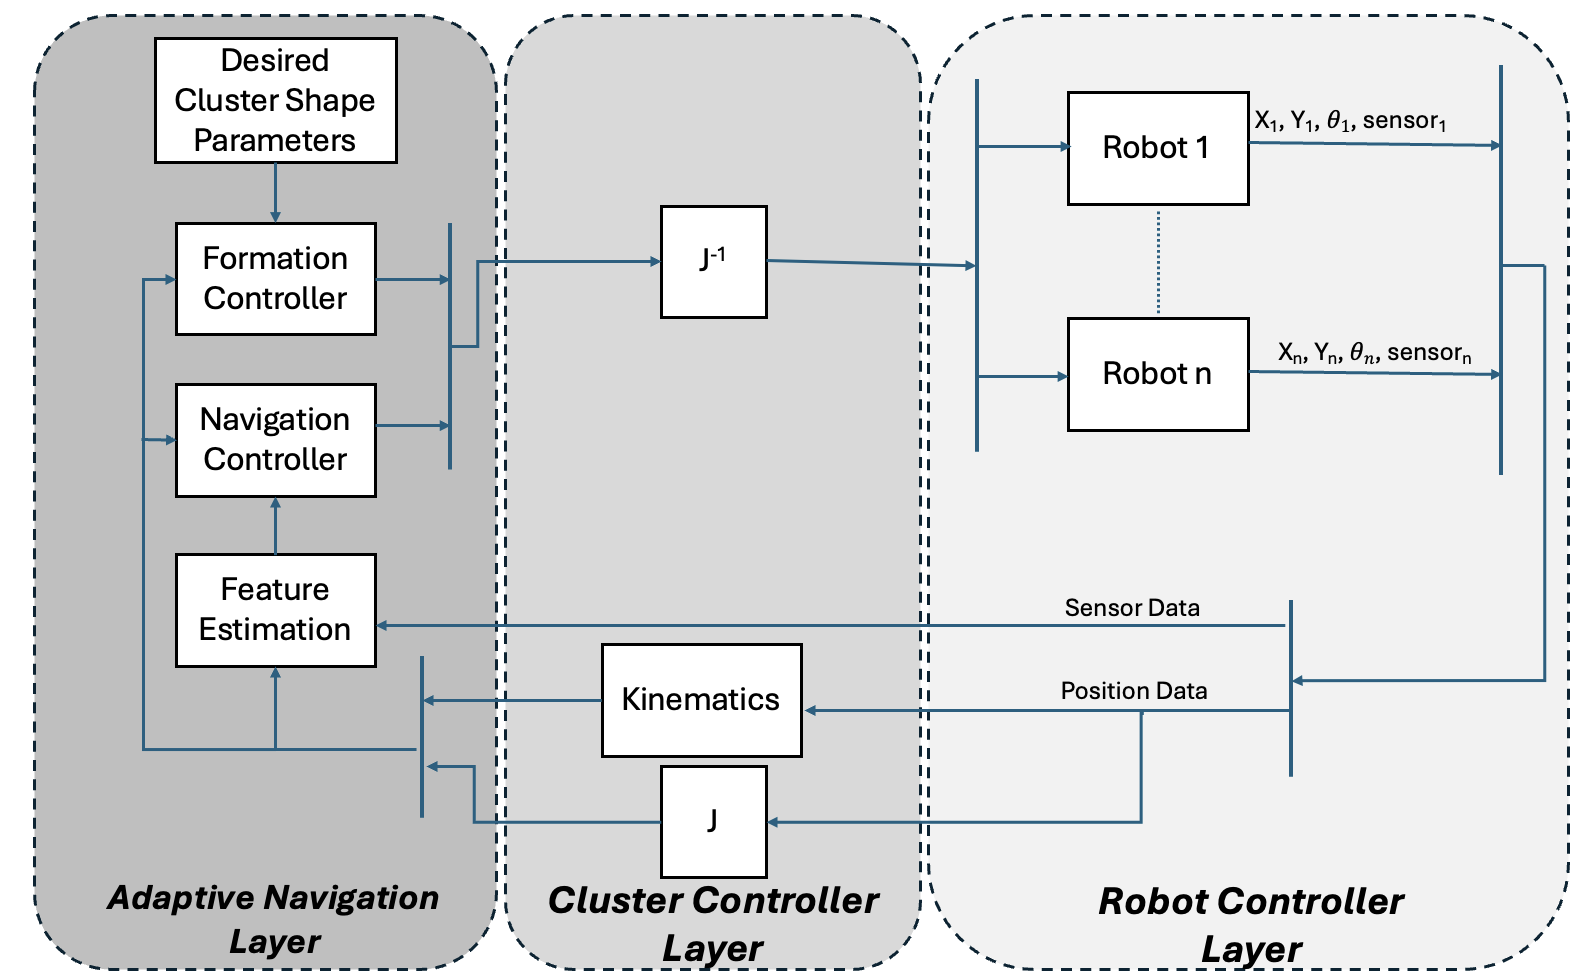
\includegraphics[width=\columnwidth]{figures/control_architecture.png}
    \caption{Three-layer control architecture. The adaptive navigation
    layer (left) estimates the field and generates the cluster command, the
    cluster controller layer (center) maps between cluster and robot space,
    and the robot controller layer (right) actuates each robot and reports
    its position and field sample.}
    \label{fig:control_architecture}
\end{figure}

\begin{figure}[!tb]
    \centering
    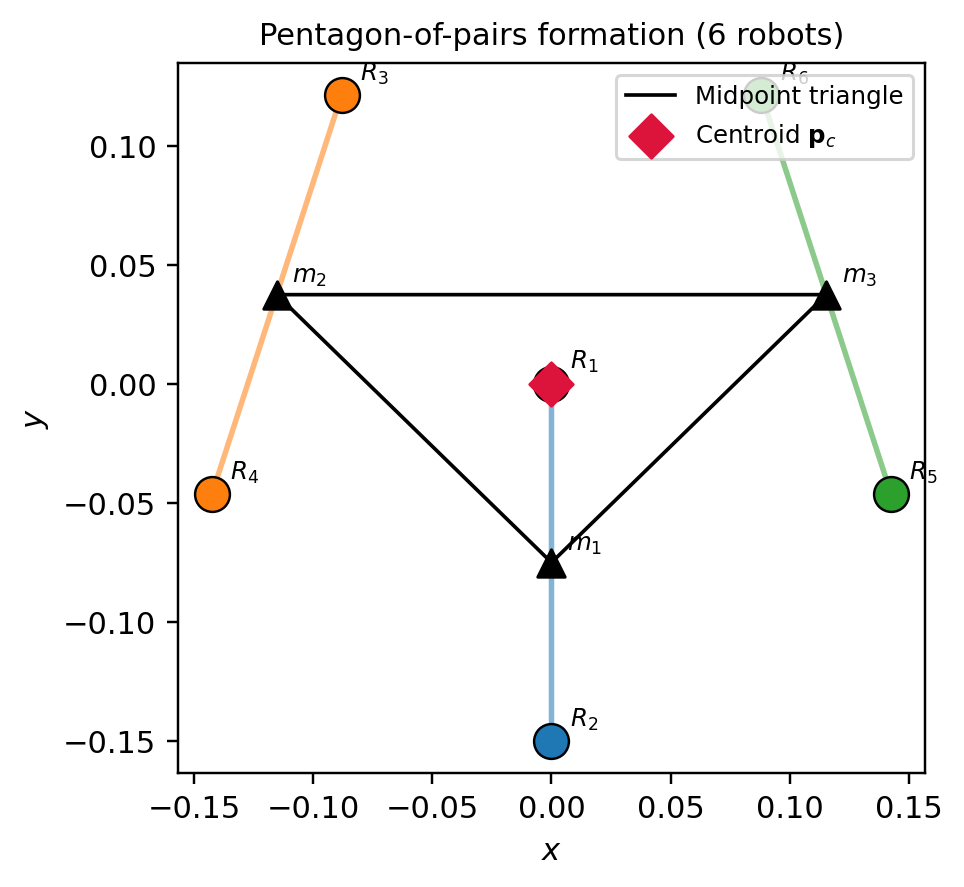
\includegraphics[width=0.8\columnwidth]{figures/pentagon_formation.png}
    \caption{Pentagon-plus-center formation. Robot 1 sits at the centroid
    $\mathbf{p}_c$ and robots 2 to 6 on a ring (dotted). The cluster
    variables shown are the pair separations $L_2$, $L_3$, $L_4$, a pair
    orientation $\theta_3$, the SAS parameters $(p, \beta, q)$ of the
    triangle of pair midpoints (squares), and the heading $\theta_c$.}
    \label{fig:pentagon}
\end{figure}

In the robot controller layer, each robot follows its velocity command
through a first-order lag, discretized at control period $\Delta t$ as the
update
$\mathbf{v} \leftarrow \alpha_{\text{mom}}\mathbf{v} + (1 -
\alpha_{\text{mom}})\mathbf{v}^{\text{des}}$ with
$\alpha_{\text{mom}} = e^{-\Delta t/\tau}$. This momentum model was
identified in \cite{10} on the Decabot indoor omnidirectional testbed
\cite{31,32}, and $\alpha_{\text{mom}} = 0.7$ at $\Delta t = 0.1$~s gives
$\tau \approx 0.28$~s, consistent with the identified lag. Each robot also
carries a speed limit and a stiction floor.

A Python simulation integrates each robot's position by explicit Euler at
the control period. Table~\ref{tab:params} gives the two operating points,
fixed across all experiments unless noted.

\begin{table}[!t]
\caption{Operating points. The double-gyre column is non-dimensional,
with one time unit equal to one second of the Decabot's identified
dynamics.}
\label{tab:params}
\centering
\begin{tabular}{llll}
\hline
Parameter & Double gyre & Ocean & Units \\
\hline
$c_{\max}$              & 0.04  & 0.033  & length/time \\
$k$                     & 3.0   & 1.94   & none \\
$\rho$                  & 0.075 & 0.098  & length (5.0 km) \\
$v_{\text{max,robot}}$  & 0.3   & 0.3    & length/time \\
$v_{\text{stiction}}$   & 0.025 & 0.002  & length/time \\
$\alpha_{\text{mom}}$   & 0.7   & 0      & none \\
$c_{\mathrm{crest}}$    & 0.1   & 0.1    & none \\
$g_\perp$              & 1.0   & 1.0    & length$^2$ \\
$q_{\mathrm{cap}}$      & 0.03  & 0.03   & none \\
\hline
\end{tabular}
\end{table}

\subsection{The $D$ Tracker}
\label{sec:sep_controller}

The $D$ tracker is built for a mountain pass in $D$. Two minima are
joined by a trench that rises to a saddle point of $D$, the crest. On the
benchmark the trench is the separatrix and the minima are the flow saddles
(Fig.~\ref{fig:dg_fields}(b)). The tracker steers the centroid onto the
trench, along it over the crest, and down toward the next minimum. It
does so with two channels, one across the trench and one along it.

Across a trench $D$ curves upward, and along it $D$ can curve either way.
The tracker reads both directions from the eigenvectors of the fitted
Hessian, $\hat{\mathbf{H}}_{D,0}\mathbf{w}_j = \lambda_j \mathbf{w}_j$,
with $\|\mathbf{w}_j\| = 1$ and $\lambda_1 \leq \lambda_2$. The
eigenvector $\mathbf{w}_2$ points across the trench and $\mathbf{w}_1$
along it, signed by $\hat{\mathbf{v}}_0^\top \mathbf{w}_1 \geq 0$ to point
downstream, where $\hat{\mathbf{v}}_0 = (\hat{a}_1, \hat{b}_1)$ is the
measured flow at the centroid. This is the height-ridge definition of a
trench \cite{33}, a curve on which the gradient is orthogonal to a Hessian
eigenvector with positive eigenvalue. The identification is exact on the
benchmark, where $\mathbf{H}_D$ is diagonal, and approximate in general.

Away from the crest, both channels take Newton steps of the fitted
quadratic along their eigenvectors. The across-trench channel steps
toward the bottom of the trench, a distance
$-\mathbf{w}_2^\top\hat{\mathbf{g}}_0/\lambda_2$ along $\mathbf{w}_2$. The
along-trench channel uses the same ratio in magnitude,
$|\mathbf{w}_1^\top\hat{\mathbf{g}}_0|/|\lambda_1|$ along $\mathbf{w}_1$,
which slows the cluster as it nears the crest.

At the crest the along-trench gradient vanishes, and the measured flow
carries the cluster over instead. The crest is a saddle point of $D$, so
the tracker detects it as a fitted saddle whose stationary point lies
inside the formation. The crest set $\mathcal{B}$ is the set of points
where
\begin{equation}
    \lambda_1\lambda_2 < 0
    \quad\text{and}\quad
    \bigl\|\hat{\mathbf{H}}_{D,0}^{-1}\,\hat{\mathbf{g}}_0\bigr\|
        < c_{\mathrm{crest}}\,\rho.
    \label{eq:band}
\end{equation}
The left side of the second test is the Newton step to the stationary
point, so $c_{\mathrm{crest}}$ is a fraction of the formation radius and
needs no knowledge of the field's scale.

Combining the two channels, the crest test selects the along-trench speed,
\begin{equation}
    v_\parallel =
    \begin{cases}
        \hat{\mathbf{v}}_0^\top \mathbf{w}_1,
            & \mathbf{p}_c \in \mathcal{B}, \\[6pt]
        \dfrac{|\mathbf{w}_1^\top \hat{\mathbf{g}}_0|}{|\lambda_1|},
            & \text{otherwise},
    \end{cases}
    \label{eq:vpar}
\end{equation}
and the centroid velocity command is
\begin{equation}
    \dot{\mathbf{p}}_c = k\Bigl[
    \underbrace{\mathrm{sat}(v_\parallel)\,\mathbf{w}_1}_{\text{along the trench}}
    + \underbrace{\mathrm{sat}\!\left(-\frac{\mathbf{w}_2^\top
      \hat{\mathbf{g}}_0}{\lambda_2}\right)\mathbf{w}_2}_{\text{across the trench}}\Bigr].
    \label{eq:d_law}
\end{equation}
Here $k$ is a navigation gain and
$\mathrm{sat}(c) = c_{\max}\tanh(c/c_{\max})$ saturates each channel at
speed $c_{\max}$, which caps the centroid speed at $\sqrt{2}\,k\,c_{\max}$.
Both branches of $v_\parallel$ are nonnegative, so the along-trench
motion never opposes the flow. The same law runs where the fitted Hessian
is definite and no trench exists, with $\mathbf{w}_1$ still the
eigenvector of the smaller eigenvalue, so the tracker needs no separate
rule there.

The tracker stops at the end of the pass with the critical point test of
\cite{10}. On the benchmark the minima of $D$ are the flow saddles, and
the test fires when the fitted flow has a saddle inside the formation,
\begin{equation}
    \det\hat{\mathbf{J}}_0 < 0
    \quad\text{and}\quad
    \bigl\|\hat{\mathbf{J}}_0^{-1}\hat{\mathbf{v}}_0\bigr\| < \rho,
    \label{eq:d_capture}
\end{equation}
where $\hat{\mathbf{J}}_0$ is the fitted Jacobian at the centroid and
$\hat{\mathbf{J}}_0^{-1}\hat{\mathbf{v}}_0$ is the Newton step to the
stagnation point. The test uses only the zeroth- and first-order
coefficients, the least noisy the fit returns. Once it passes, the tracker
holds for the rest of the run with the attraction law of \cite{10},
\begin{equation}
    \dot{\mathbf{p}}_c = k\,\mathrm{sat}\bigl(-\hat{\mathbf{J}}_0^{-1}\hat{\mathbf{v}}_0\bigr),
    \label{eq:d_hold}
\end{equation}
with $\mathrm{sat}$ applied to each component, which steers the centroid to
the fitted stagnation point from the same coefficients as the test. Both
read the measured flow, so neither is objective.

The across-trench channel drives the cluster to the fitted trench bottom
with the command $\mathbf{w}_2^\top\dot{\mathbf{p}}_c = k\,\mathrm{sat}(e)$,
where $e = -\mathbf{w}_2^\top\hat{\mathbf{g}}_0/\lambda_2$ is the signed
distance to the trench bottom. Assuming a stationary estimate, the
Lyapunov function $V = \tfrac{1}{2}e^2$ yields $\dot{V} = -k\,e\,\mathrm{sat}(e) < 0$ for
$e \neq 0$, guaranteeing convergence. This descent assumes positive
curvature ($\lambda_2 > 0$), which holds intrinsically unless inverted by
noise.

\subsection{The $s_1$ Tracker}
\label{sec:s1_controller}

The fitted $\hat{s}_1$ is concave for every field and formation
(Section~\ref{sec:surrogates}). It never shows the upward curvature a
trench has across it, and the Newton step that returns the $D$ tracker to
its trench has no counterpart here. The tracker instead builds both
channels from $\nabla\hat{s}_1$ and the strain eigenframe.

The trench tangent is a strain eigenvector (Section~\ref{sec:surrogates}),
and the tracker must choose between $\mathbf{e}_1$ and $\mathbf{e}_2$ at
every step. On the trench the transverse derivative of $s_1$ vanishes, so
$\nabla\hat{s}_1$ lies nearly along the trench away from a stationary
point. The tangent is the eigenvector most nearly parallel to it, signed
against a reference,
\begin{equation}
    \mathbf{t}_{\mathrm{raw}} =
    \arg\max_{\mathbf{e} \in \{\mathbf{e}_1, \mathbf{e}_2\}}
    \bigl\lvert \nabla\hat{s}_1^\top \mathbf{e} \bigr\rvert,
    \qquad
    \mathbf{t} = \mathrm{sgn}\bigl(\mathbf{t}_{\mathrm{ref}}^\top
    \mathbf{t}_{\mathrm{raw}}\bigr)\,\mathbf{t}_{\mathrm{raw}},
    \label{eq:tangent_select}
\end{equation}
where $\mathbf{t}_{\mathrm{ref}}$ is the previous step's tangent
(Fig.~\ref{fig:s1_channels}(a)). On a trench that is not an OECS, the
rule takes the nearer eigenvector. The first ride step has no previous
tangent, so the measured flow $\hat{\mathbf{v}}_0$ serves as
$\mathbf{t}_{\mathrm{ref}}$. Because the measured flow is not objective,
it seeds the ride direction only once.

From the first step, the command pairs a constant-speed ride along
$\mathbf{t}$ with gradient descent across the trench,
\begin{equation}
    \dot{\mathbf{p}}_c = k\Bigl[
    \underbrace{\mathrm{sat}(c_{\max})\,\mathbf{t}}_{\text{along the trench}}
    + \underbrace{\mathrm{sat}\bigl(-g_\perp\,\mathbf{t}_\perp^\top
      \nabla\hat{s}_1\bigr)\,\mathbf{t}_\perp}_{\text{across the trench}}\Bigr],
    \label{eq:s1_law}
\end{equation}
with transverse gain $g_\perp$ and $\mathbf{t}_\perp$ the unit normal to
$\mathbf{t}$. The cluster rides at speed $k\,c_{\max}\tanh 1$ throughout.
The across-trench channel sees only the component of $\nabla\hat{s}_1$
along $\mathbf{t}_\perp$ (Fig.~\ref{fig:s1_channels}(b)), so the cluster
descends only across the trench.

The ride speed does not depend on the slope, so the cluster crosses the
crest without the crest test the $D$ tracker needs. In incompressible
flow $s_1 = -r \leq 0$, which reaches zero only at an isotropic point,
where the strain vanishes. Such a point is in general an isolated peak,
so the crest is a smooth saddle with $r > 0$. There $\nabla\hat{s}_1$
vanishes, and the tangent rule is least reliable, as it is near a
minimum. In special flows, such as one whose shear strain vanishes
identically, the isotropic points form curves, and the crest can sit on
one at a kink of $s_1$.

The tangent changes eigenvector only at an isotropic point, and the rule
follows the swap with no dedicated test, since $\nabla\hat{s}_1$ stays
large on either side of the kink. On the benchmark,
$\mathbf{S} = \mathrm{diag}(u_x, -u_x)$ has its eigenvectors on the
coordinate axes wherever $u_x \neq 0$. On the upper segment of the
separatrix $u_x < 0$, so the trench follows $\mathbf{e}_2$ and is an
attracting OECS. On the lower segment $u_x > 0$, so it follows
$\mathbf{e}_1$ and is a repelling OECS. The two meet at the origin, an
isotropic point of $\mathbf{S}$ where the crest sits at a kink.

The tracker stops at a minimum by a gradient test. The concave fit cannot
certify a minimum, but the fitted gradient tracks the true gradient even
where the fitted curvature has the wrong sign. Each end of the trench is
a true two-dimensional minimum of $s_1$, so a gradient that is small
against the depth suffices. Capture requires $\hat{s}_1 < 0$ and
\begin{equation}
    q = \frac{\rho\,\|\nabla\hat{s}_1\|}{|\hat{s}_1|} < q_{\mathrm{cap}},
    \label{eq:s1_capture}
\end{equation}
where $q$ is the fraction by which $\hat{s}_1$ changes across the
footprint. The ratio is dimensionless, so $q_{\mathrm{cap}}$ needs no
knowledge of the field's strain rate. It is large along the ride and
wherever $\hat{s}_1$ nears zero, as at an isotropic point or a gyre
center, and small only near a minimum. Once the test passes, the tracker
drops the ride term and descends $\hat{s}_1$ for the rest of the run with
$\dot{\mathbf{p}}_c = -k\,\mathrm{sat}(g_\perp\nabla\hat{s}_1)$. Here
$\mathrm{sat}$ saturates the vector's magnitude at $c_{\max}$ and
preserves its direction, which keeps the descent independent of the
coordinate axes. If noise trips the test early on the trench, the descent
still carries the cluster down the trench to the minimum.

\begin{figure}[!tb]
    \centering
    \includegraphics[width=\columnwidth]{figures/s1_channels.png}
    \caption{The two channels of the $s_1$ tracker, on the benchmark
    trench at $x = 0$. (a) Tangent selection. At each sample the strain eigenframe is
    drawn, the selected eigenvector heavy and the rejected one light,
    with $\nabla\hat{s}_1$ in orange. The argmax takes
    $\mathbf{e}_2$ on the attracting segment and $\mathbf{e}_1$ on the
    repelling segment, swapping through the isotropic point at the origin.
    (b) The command. Travel along $\mathbf{t}$ is open loop at cruise
    speed, while descent uses only the component of $\nabla\hat{s}_1$
    along $\mathbf{t}_\perp$, so the cluster descends only across the
    trench.}
    \label{fig:s1_channels}
\end{figure}

The across-trench channel drives the cluster to the trench using the
command $\mathbf{t}_\perp^\top\dot{\mathbf{p}}_c =
-k\,\mathrm{sat}(g_\perp\mathbf{t}_\perp^\top\nabla\hat{s}_1)$. For signed
transverse distance $n$, assuming realized kinematics and an accurate
gradient fit, the Lyapunov function $V = \tfrac{1}{2}n^2$ yields
$\dot{V} = -k\,n\,\mathrm{sat}(g_\perp\mathbf{t}_\perp^\top\nabla\hat{s}_1) < 0$
for $n \neq 0$, guaranteeing local convergence (and ultimate boundedness
under disturbances below $k\,c_{\max}$). Because no fitted curvature
enters, this descent relies only on the true upward curvature of the
trench, which holds intrinsically, even at smooth crests, unless an
intersecting curve of isotropic points flattens the trench, leaving the
tangent ride to carry the cluster across alone.


\section{Double-Gyre Benchmark}
\label{sec:dg_bench}

\subsection{Setup}

The double-gyre experiments use the steady field of
Section~\ref{sec:dg_example} and the nominal formation, with ring radius
$\rho = 0.075$. Trials vary only the initial heading, set to zero in the
noise-free runs and drawn uniformly from $[0, 2\pi)$ in the Monte Carlo
sweeps. All trials run for up to 500 steps.

Performance is scored on acquisition, saddle capture, and straddle
retention. A run acquires the separatrix at the first of ten consecutive
steps with its centroid within 0.05 of $x = 0$. Noise-free trials stop once
the centroid has stayed within 0.06 of a flow saddle for 20 consecutive
steps, while noisy trials succeed if the centroid comes within 0.06 of the
far saddle $\mathbf{p}^*_1 = (0, -0.5)$. In a separate check of 1260 longer
trials at three noise levels, every trial but one that reached a saddle
also held it for 20 consecutive steps. Because losing the straddle is the
failure \cite{26} reports, we measure noise tolerance by retention, the
fraction of trials that succeed and never stop straddling the separatrix
after their first straddle.

\subsection{Clean Runs}
\label{sec:disc_clean}

\begin{figure}[!tb]
    \centering
    \includegraphics[width=1.0\columnwidth]{figures/traverse_vs_logic_c_seven.png}
    \caption{$s_1$ tracker versus $D$ tracker from seven matched starts
    ($\bullet$), noise-free, at S1 $(-0.10, 0.30)$, S2 $(0.15, 0.25)$, S3 $(0, 0.35)$,
    S4 $(0, 0)$, S5 $(0, -0.25)$, S6 $(0.15, -0.15)$, and S7 $(0.10, -0.20)$. From above the origin both
    traverse the separatrix through the isotropic point there. Both
    trackers capture and hold the far saddle ($\times$), ending at the
    squares.}
    \label{fig:traverse_vs_logic_c}
\end{figure}

\begin{figure}[!tb]
    \centering
    \includegraphics[width=1.0\columnwidth]{figures/separatrix_formation_seven.png}
    \caption{The six robots from start S1 (star) under both trackers,
    zoomed to the separatrix $x = 0$ (dashed). Thin lines are robot
    paths and the heavy line is the centroid. Outlines mark the
    pentagon-plus-center formation at the start, during the ride, and at
    the far saddle ($\times$).}
    \label{fig:formation}
\end{figure}

Without noise, both trackers acquire the separatrix, traverse it in the
same direction, and capture the far saddle from all seven matched starts
(Fig.~\ref{fig:traverse_vs_logic_c}). Three starts lie on the separatrix,
at heights $0.35$, $0$, and $-0.25$. Four lie off it by $1.3\rho$ or
$2\rho$, two above the origin and two below, and none of these straddles
the separatrix at the first step. Both trackers acquire the separatrix
from all seven starts in 0 to 10 steps. Runs from above the origin then
ride the upper segment to the isotropic point at the origin and continue
onto the lower segment, with the formation straddling the separatrix
throughout (Fig.~\ref{fig:formation}). A run acquiring above the origin
therefore rides an attracting OECS to the origin and continues onto a
repelling one on the same primitive and scalar trench, and the $s_1$
tracker crosses the origin on ordinary tangent selection.

Both hold the far saddle $\mathbf{p}^*_1 = (0, -0.5)$ in all seven runs
(Fig.~\ref{fig:traverse_vs_logic_c}). The $s_1$ tracker settles within
0.014 of it and the $D$ tracker within 0.004 to 0.006.

\subsection{Behavior Under Noise}
\label{sec:disc_noise}

\begin{figure}[!tb]
    \centering
    \includegraphics[width=\columnwidth]{figures/noise_seven_starts_col.png}
    \caption{Far-saddle success of both trackers from the seven starts of
    Fig.~\ref{fig:traverse_vs_logic_c}, one per row, $10^4$ trials per point,
    with each tracker's retention, the fraction of trials that succeed and
    keep the straddle, dashed. S1 and S2 start off the separatrix above the origin, S3, S4, and S5
    on it, and S6 and S7 off it below the origin. Each inset marks the start
    (dot) in the basin, with the separatrix dashed and the far saddle
    $\mathbf{p}^*_1$ starred. (a) Against $\sigma_{uv}$, $\sigma_p = 0$. (b) Against
    $\sigma_p$, $\sigma_{uv} = 0$.}
    \label{fig:flip_resolution}
\end{figure}

Both primitives sweep measurement and position noise separately from the
seven starts of Fig.~\ref{fig:traverse_vs_logic_c}, at $10^4$ trials per
noise level from independent headings (Fig.~\ref{fig:flip_resolution}).
Without noise, both trackers
reach $\mathbf{p}^*_1$ in all $10^4$ trials from every start.

Both trackers degrade smoothly as noise grows, with no threshold at which
either suddenly fails. From S3, the $D$ tracker's retention
falls from 99.4\% at $\sigma_{uv} = 0.0015$ to 23\% at $\sigma_{uv} = 0.03$,
while the $s_1$ tracker's falls from 85\% at $\sigma_{uv} = 0.00075$ to
under 1\% at $\sigma_{uv} = 0.004$.

Both trackers fail at high noise for the same reason. Each steers on the
second-order coefficients of the fit, which carry the most noise because
the fit recovers them from velocity differences divided by $\rho^2$. For
this formation each pure second derivative carries a standard deviation of
$2.53\,\sigma_{uv}/\rho^2$. At $\rho = 0.075$ this noise matches the
largest second derivative in the field, $\pi^3 A \approx 3.1$, near
$\sigma_{uv} = 0.007$. Beyond this level the fit cannot resolve even
the strongest curvature in the field, and by $\sigma_{uv} = 0.01$ neither
tracker retains more than 65\% of its trials from any start.

The $D$ tracker tolerates more noise than the $s_1$ tracker from every
start, under both noise types. Against measurement noise, the level at
which its retention falls to 50\% is 5.4 to 5.8 times the $s_1$ tracker's
above the origin, 4.2 times at it, and 1.1 to 1.2 times from S6 and S7.
From S5 its retention never falls to 50\%. The
order reverses only at high noise from S6 and S7, where the two retention
curves cross near $\sigma_{uv} = 0.006$.

The $s_1$ tracker fails in two ways. The main one is a reversal, in which
the cluster turns around on the separatrix and rides it the wrong way. At
$\sigma_{uv} = 0.002$, 97 to 98\% of the $s_1$ trials that
miss $\mathbf{p}^*_1$ end at $\mathbf{p}^*_2$, from every start.
Even runs from below the origin therefore climb past it against the flow.
Reversals come from how the tracker keeps its direction. The $D$ tracker
re-signs its direction every cycle against the measured flow. That flow is
not objective, so the $s_1$ tracker instead carries its sign forward from
step to step. Near the saddles, the along-trench slope
$\pi^3 A|\sin\pi y_f|$ that tangent selection relies on goes to zero. One
noisy step there can select the transverse eigenvector, after which the
next step's sign is arbitrary. The $s_1$ capture holds whichever saddle
the ride reaches, including $\mathbf{p}^*_2$ after a reversal. The second
failure is subtler, reaching
$\mathbf{p}^*_1$ but losing the straddle on the way. From S5 at
$\sigma_{uv} = 0.01$, 77\% of the $s_1$ tracker's trials reach
$\mathbf{p}^*_1$ but only 33\% keep the straddle. For the $D$ tracker the
two rates differ by at most 6 percentage points up to
$\sigma_{uv} = 0.005$.

The $D$ tracker's lower tolerance from S6 and S7 comes from the fitted
Hessian becoming definite before the cluster reaches the separatrix.
Because the fitted eigenvalues shrink toward the saddles, noise can make
$\hat{\mathbf{H}}_{D,0}$ definite during acquisition. At
$\sigma_{uv} = 0.005$ this occurs in 92\% and 83\% of trials from S6 and
S7, and only 45\% and 51\% of those trials go on to reach
$\mathbf{p}^*_1$, against 85\% for the rest. From S1 and S2 the fitted
Hessian becomes definite in 75\% and 83\% of trials without changing
success. Runs from S1 and S2 meet the separatrix inside $|y| < 0.25$,
where the true $\mathbf{H}_D$ is indefinite, while runs from S6 and S7
meet it near $y = -0.30$, where it is definite.

\subsection{Behavior Under a Rotating Observer}
\label{sec:rotating}

\begin{figure}[!tb]
    \centering
    \includegraphics[width=0.82\columnwidth]{figures/objectivity_rotating.png}
    \caption{Rotating-observer trial from S1 (star), $10^4$ trials per
    frame, pulled back to inertial coordinates. Lines are mean paths with
    one standard deviation shaded, and squares are median final
    positions. Pentagons show heading-zero runs at $\Omega = \pm 0.23$.
    The $D$ tracker leaves the separatrix (dashed) toward a side set by
    the sense of rotation, while the $s_1$ tracker's paths coincide.}
    \label{fig:oecs_objectivity}
\end{figure}

A cluster can sense the water without error and still see the flow from a
rotating frame. This happens when each robot senses water velocity relative
to itself and adds its own velocity, differenced from position fixes
expressed in drifting axes. The flow the cluster measures is then
\[
\mathbf{v}'(\mathbf{p}', t) =
\mathbf{Q}\mathbf{v}(\mathbf{Q}^\top \mathbf{p}') + \Omega\,(-y', x')^\top ,
\]
the physical flow seen in rotated axes plus the transport velocity of a
frame rotating at rate $\Omega$, clockwise for $\Omega > 0$.

Both trackers start from S1 on the noise-free double gyre and run in the
inertial frame and in frames rotating at $\Omega = \pm 0.10$ and
$\pm 0.23$, with $10^4$ trials of random heading per frame. A trial stops
once its centroid, pulled back to inertial coordinates, stays within
$0.2\rho$ of its mean over 20 steps, or after 500 steps. The frame carries each point of the flow at speed
$|\Omega|\lVert\mathbf{p}\rVert$, largest at $\mathbf{p}^*_1$, where it
is $0.5|\Omega|$. The $s_1$ tracker's capture saturates its command at
$k\,c_{\max} = 0.12$, so it can hold $\mathbf{p}^*_1$ only while
$|\Omega| < 0.24$. The $D$ tracker's capture saturates each channel and
can reach $\sqrt{2}\,k\,c_{\max}$, giving it more speed near this bound.

The $s_1$ tracker follows the same path in every frame
(Fig.~\ref{fig:oecs_objectivity}, right). Its median largest offset from
the separatrix is 0.011 in the inertial frame and at most
0.017 in the rotating frames, and no trial loses the straddle. Its
channels and capture test are built from quantities a rotation leaves
invariant, so its command co-rotates with the frame. Its one
non-objective input is the tangent seed, on which both frames agree from
S1.

The $D$ tracker's path depends on the frame
(Fig.~\ref{fig:oecs_objectivity}, left). Its median largest offset is
0.010 in the inertial frame, 0.037 at $|\Omega| = 0.10$, and
0.084 at $|\Omega| = 0.23$, and it varies by less than 0.002
across headings. At $|\Omega| = 0.23$ every trial loses the straddle, for
a median of 40 steps, the failure \cite{26} reports. Reversing the
sense of rotation mirrors the path, since the double gyre is symmetric
about the separatrix.

The $D$ tracker departs because the frame's added vorticity $2\Omega$
shifts $D'$ by (\ref{eq:D_not_objective}). On the separatrix the added
term $\Omega\omega$ is zero, but its transverse gradient
$\partial_x\omega = 2\pi^3 A\sin\pi y_f$ is not. Against the trench's
transverse curvature $2\pi^6 A^2$, it moves the trench by
$\Omega\sin(\pi y_f)/(\pi^3 A)$, which is 0.032 and 0.074 at the
origin for the two rates. The transport velocity also moves the
stagnation point of $\hat{\mathbf{v}}_0$ about $0.5|\Omega|/(\pi^2 A)$
from $\mathbf{p}^*_1$. At $|\Omega| = 0.10$ the $D$ tracker captures and
holds this shifted point, a median 0.067 from $\mathbf{p}^*_1$
against 0.013 for the $s_1$ tracker. At $|\Omega| = 0.23$ the
shift exceeds $\rho$, and its capture test passes in only 1\% of
trials.

\section{Santa Barbara Channel Trial}
\label{sec:ocean}

\subsection{Setup}
\label{sec:ocean_sim}

The ocean experiment uses the public HFRNet U.S.~West Coast surface-current
product for the Santa Barbara Channel, on its 2~km grid \cite{34,38}. We
use the record of \cite{26}, 29 hourly frames from May 16, 2012 08:00 GMT
to May 17, 2012 12:00 GMT, in the same channel and month used by
\cite{29}. Radar coverage is partial, with 74 to 87\% of the water cells
valid in each frame. Missing cells, including land inside the coverage, are
filled by linear interpolation across the valid ones, and the field is zero
beyond the valid data. Between grid points and frames the field is
interpolated bilinearly in space and linearly in time.

The simulation runs in world coordinates on $[-0.65, 0.65]^2$, mapped onto
a square centered on $(34.2^{\circ}\mathrm{N}, 120.4^{\circ}\mathrm{W})$.
One length unit is $L_w = 51.4$~km and one time unit is 6000~s. With
longitude scaled by $\cos(34.2^{\circ})$ the map is a uniform dilation, so
the zero sets, trenches, and eigenframe are the physical ones. Each control
step of $\Delta t = 0.1$ advances the field by 600~s, and the 168-step trial
covers the record. With one control cycle every ten minutes any vessel
time constant is negligible, and $\alpha_{\text{mom}} = 0$. The
commanded-speed cap $\sqrt{2}\,k\,c_{\max}$ is then 0.78~m/s, within reach
of a small autonomous surface vessel but above a buoyancy glider. Both
trackers start north of the channel entrance at
$(34.38^{\circ}\mathrm{N}, 120.41^{\circ}\mathrm{W})$ with heading
$335^\circ$. A run ends at landfall, the first step at which any robot lies
over land on the Natural Earth 1:10 million coastline, or at the end of the
28-h record.

An offline FTLE field serves as the Lagrangian reference \cite{17} and is
available to neither controller. It advects a seed grid four times finer
than the data grid through the same field by fourth-order Runge-Kutta at
600~s steps, with land held at zero velocity, over $33.8$ to
$34.7^{\circ}$N and $119.7$ to $120.7^{\circ}$W. Ridge points are the
water points at or above the 95th percentile of the 24-h forward FTLE field
anchored at the record start (Fig.~\ref{fig:ocean_ftle}). Recomputing a
12-h FTLE field at four anchor times across the record shows that this
dominant ridge persists while the finer structure downstream evolves.

The pentagon is enlarged to $\rho = 0.098$, 1.3 times the nominal radius
and 5.0~km at this site (Table~\ref{tab:params}). Inside one grid cell the
interpolated field is bilinear, so a quadratic fit sees the field's
curvature only across several cells, and the enlargement spans about five
grid cells instead of fewer than four. The radius $\rho$ and gain $k$ are
tuned against the FTLE reference, as they set when the cluster reaches the
bifurcation of the evolving ridge and therefore which branch it meets.

\subsection{Results}
\label{sec:disc_ocean}

\begin{figure*}[!tb]
    \centering
    \includegraphics[width=\textwidth]{figures/ocean_progression_2km.png}
    \caption{$D$ and $s_1$ tracker paths from a single shared start at
    (a) 7, (b) 14, (c) 21, and (d) 28~h, each drawn up to that time, with
    dots marking the current positions. The background is the 24-h forward
    FTLE field computed offline from the same 2~km data and anchored at the
    record start. Both follow the dominant ridge from the channel entrance
    to the bifurcation and take the same branch past it.}
    \label{fig:ocean_ftle}
\end{figure*}

Both trackers follow the dominant ridge of the forward FTLE field from the
channel entrance to the bifurcation and take the same branch past it
(Fig.~\ref{fig:ocean_ftle}), with no changes to the primitives at the
ocean operating point of Table~\ref{tab:params}. This agreement is not built
in, as the field is divergent and not vorticity-free. Along both paths,
however, the fit is strain-dominated, with $\hat{D} < 0$ on about 80\% of
steps and a median $|\hat{\omega}|/2\hat{r}$ of 0.15 to 0.20 from 7 to 21~h.
$D$ is then close to $s_1 s_2 = \mu^2 - r^2$, where divergence enters only
as $\mu^2$, a tenth to a fifth of $r^2$. The paths average within 1.3~km of
each other.

The $s_1$ tangent also types the structure. From 7 to 14~h it was
$\mathbf{e}_2$ on 34 of 42 steps, an attracting OECS where floating
material collects \cite{12}. From 14 to 21~h it was $\mathbf{e}_1$ on 37 of
42 steps, a repelling OECS where the trench is also a ridge of $s_2$ (on
58\% of those steps).

The trackers diverge in speed early in the trial. From 2 to 6.5~h the
$s_1$ tracker crossed a rotation-dominated patch ($\hat{D} > 0$ on 70\% of
steps), switching tangents 12 times in 27 steps and making 2.1~km of net
progress against 8.4~km for the $D$ tracker. Once past it, both kept pace
along the corridor, with an overall mean distance to the ridge of 1.6~km
for the $D$ tracker and 2.1~km for the $s_1$ tracker. The $D$ tracker
reaches land at 23~h. The $s_1$ tracker reached the southern channel
($34.21^{\circ}\mathrm{N}$) 7~h later, where fitted strain had halved
\cite{26}; its ridge distance grew to 3.8~km and it remained at sea at
28~h.

\section{Limitations and Future Work}
\label{sec:disc_limits}

Cluster space control is centralized and needs global state and reliable
high-bandwidth communication \cite{30}. Unlike distributed or
event-triggered consensus protocols \cite{35}, the estimator gathers all six
readings on one processor each step. The claims here are for small clusters
in a limited workspace with ample bandwidth.

The $s_1$ tracker's tangent selection weakens near the saddles, and its
passage through the origin rests on the benchmark's vanishing shear
strain. Without it the strain eigenvector
can tilt off the trench, the open-loop ride along $\mathbf{t}$ then
pushes the cluster across it, and the crest becomes a smooth saddle where
tangent selection rests on a weak signal.

The $D$ tracker relies on properties of the fitted quadratic and the
inertial frame. It assumes the crest is a saddle of the fitted $D$, which
is untested off the benchmark, and its traversal on the benchmark rests on
the third-derivative terms the fitted Hessian omits. Under noise, the
fitted Hessian can also become definite before acquisition. Finally, a
rotating observer shifts the $D'$ landscape and the crest, and the capture
test and hold read the measured flow, so the tracker is not objective.

The evaluation here is limited to kinematic simulation without flow
advection. The ocean trial is a single record sampled without added noise,
and in general neither instantaneous Eulerian field is guaranteed to mark a
Lagrangian material transport structure \cite{18}. No head-to-head against
\cite{26,27,28} or \cite{29} was run because their robots are advected by
the flow and one simulator cannot host both models. The no-advection
premise is exact for the planned Decabot hardware follow-on, where the
field is encoded rather than physically experienced \cite{32}, but remains
untested in a physical flow.

Future work targets three extensions. First, a fit from more than six
robots becomes least squares, which averages the measurement noise and
leaves a residual that estimates it online. A cluster could then detect the
high-noise regime in which neither tracker is reliable. Second, the
$s_1$ tracker could take as its tangent the strain eigenvector nearest the
previous tangent, holding the previous tangent where the eigenframe is
unresolved. That rule does not rest on the along-trench slope, which
vanishes near the saddles where reversals concentrate. Finally, a cubic fit
from ten robots off any common cubic curve would take the progression from
the linear fit of \cite{10} to the quadratic fit here one order further. It
would recover the third derivatives on which the true $\mathbf{H}_D$ and
the transverse curvature of an $s_1$ trench depend.

\section{Conclusion}

This paper has shown that six robots sampling at once can fit a local
quadratic model of a planar flow, which gives the velocity gradient as a
field over the formation. Two surrogate fields read from that fit, the
Jacobian determinant $D$ and the smaller strain eigenvalue $s_1$, mark
coherent structures of the flow as trenches. On each field we built an
adaptive navigation primitive that acquires and rides those trenches from
instantaneous measurements, with no integration horizon and no
pre-straddling. Without noise, both acquire and traverse the
double-gyre separatrix from every start and hold the far saddle. The $D$
tracker withstands more measurement and position noise than the $s_1$
tracker from every start tested. The $s_1$ tracker is objective past its
one seed step, and it alone holds the same path under a rotating observer.
A cluster with an absolute heading reference, such as a compass or GNSS,
should therefore carry the $D$ tracker, and one whose flow estimate
carries its own rotation should carry the $s_1$ tracker.

\begin{thebibliography}{99}
\itemsep 0pt plus 0.2pt
\parskip 0pt
\bibitem{1} J. Cortés and M. Egerstedt, ``Coordinated control of multi-robot
systems: A survey,'' \textit{SICE J. Control Meas. Syst. Integr.},
vol. 10, no. 6, pp. 495--503, 2017.

\bibitem{2} T. Adamek, C. A. Kitts, and I. Mas, ``Gradient-based cluster space
navigation for autonomous surface vessels,'' \textit{IEEE/ASME Trans.
Mechatronics}, vol. 20, no. 2, pp. 506--518, 2015.

\bibitem{3} C. A. Kitts, R. T. McDonald, and M. A. Neumann, ``Adaptive
navigation control primitives for multirobot clusters: Extrema finding,
contour following, ridge/trench following, and saddle point station keeping,''
\textit{IEEE Access}, vol. 6, pp. 17625--17642, 2018.

\bibitem{4} R. T. McDonald et al., ``Navigation of
scalar fronts with multirobot clusters in simulation and experiment,''
\textit{IEEE Syst. J.}, vol. 14, no. 3, pp. 3755--3766, 2020.

\bibitem{5} L. Briñón-Arranz, A. Renzaglia, and L. Schenato, ``Multirobot
symmetric formations for gradient and Hessian estimation with application to
source seeking,'' \textit{IEEE Trans. Robot.}, vol. 35, no. 3,
pp. 782--789, 2019.

\bibitem{6} P. Ögren, E. Fiorelli, and N. E. Leonard, ``Cooperative control
of mobile sensor networks: Adaptive gradient climbing in a distributed
environment,'' \textit{IEEE Trans. Autom. Control}, vol. 49, no. 8,
pp. 1292--1302, 2004.

\bibitem{7} R. T. McDonald, C. A. Kitts, and M. A. Neumann, ``Experimental
implementation and verification of scalar field ridge, trench, and saddle
point maneuvers using multirobot adaptive navigation,'' \textit{IEEE Access},
vol. 7, pp. 62950--62961, 2019.

\bibitem{8} A. Okubo, ``Horizontal dispersion of floatable particles in the
vicinity of velocity singularities such as convergences,'' \textit{Deep-Sea
Res.}, vol. 17, no. 3, pp. 445--454, 1970.

\bibitem{9} P. Keramea, K. Spanoudaki, G. Zodiatis, G. Gikas, and
G. Sylaios, ``Oil spill modeling: A critical review on current trends,
downscaling, and applications,'' \textit{J. Mar. Sci. Eng.}, vol. 9,
no. 2, art. 181, 2021.

\bibitem{10} C. Waight and C. A. Kitts, ``Adaptive navigation of multirobot
systems to critical points in 2D vector fields,'' submitted for publication.

\bibitem{11} T. Peacock and G. Haller, ``Lagrangian coherent structures: The
hidden skeleton of fluid flows,'' \textit{Phys. Today}, vol. 66, no. 2,
pp. 41--47, 2013.

\bibitem{12} M. Serra et al., ``Search and rescue at sea aided by hidden flow
structures,'' \textit{Nat. Commun.}, vol. 11, no. 1, p. 2525, 2020.

\bibitem{13} J. Das et al., ``Coordinated sampling of dynamic oceanographic
features with underwater vehicles and drifters,'' \textit{Int. J. Robot.
Res.}, vol. 31, no. 5, pp. 626--646, 2012.

\bibitem{14} S. McCammon et al., ``Ocean front detection and tracking using a
team of heterogeneous marine vehicles,'' \textit{J. Field Robot.}, vol. 38,
no. 6, pp. 854--881, 2021.

\bibitem{15} S. R. Ramp et al., ``Preparing to predict: the second autonomous
ocean sampling network (AOSN-II) experiment in the Monterey Bay,''
\textit{Deep-Sea Res. II}, vol. 56, no. 3-5, pp. 68--86, 2009.

\bibitem{16} G. Haller and G. Yuan, ``Lagrangian coherent structures and mixing
in two-dimensional turbulence,'' \textit{Physica D}, vol. 147, no. 3-4,
pp. 352--370, 2000.

\bibitem{17} S. C. Shadden, F. Lekien, and J. E. Marsden, ``Definition and
properties of Lagrangian coherent structures from finite-time Lyapunov
exponents in two-dimensional aperiodic flows,'' \textit{Physica D}, vol. 212,
no. 3-4, pp. 271--304, 2005.

\bibitem{18} G. Haller, ``Lagrangian coherent structures,'' \textit{Annu. Rev.
Fluid Mech.}, vol. 47, pp. 137--162, 2015.

\bibitem{19} M. Serra and G. Haller, ``Objective Eulerian coherent
structures,'' \textit{Chaos}, vol. 26, no. 5, p. 053110, 2016.

\bibitem{20} P. J. Nolan, M. Serra, and S. D. Ross, ``Finite-time Lyapunov
exponents in the instantaneous limit and material transport,''
\textit{Nonlinear Dyn.}, vol. 100, no. 4, pp. 3825--3852, 2020.

\bibitem{21} T. D. Harms, S. L. Brunton, and B. J. McKeon, ``Lagrangian
gradient regression for the detection of coherent structures from sparse
trajectory data,'' \textit{R. Soc. Open Sci.}, vol. 11, no. 9,
p. 240586, 2024.

\bibitem{22} J. Weiss, ``The dynamics of enstrophy transfer in two-dimensional
hydrodynamics,'' \textit{Physica D}, vol. 48, no. 2-3, pp. 273--294, 1991.

\bibitem{23} J. C. R. Hunt, A. A. Wray, and P. Moin, ``Eddies, streams, and
convergence zones in turbulent flows,'' in \textit{Proc. Summer Program,
Center Turbul. Res.}, Rep. CTR-S88, pp. 193--208, 1988.

\bibitem{24} B.-L. Hua and P. Klein, ``An exact criterion for the stirring
properties of nearly two-dimensional turbulence,'' \textit{Physica D}, vol. 113,
no. 1, pp. 98--110, 1998.

\bibitem{25} C. Dong et al., ``Oceanic mesoscale eddies,''
\textit{Ocean-Land-Atmos. Res.}, vol. 4, p. 0081, 2025.

\bibitem{26} M. Michini, M. A. Hsieh, E. Forgoston, and I. B. Schwartz,
``Robotic tracking of coherent structures in flows,'' \textit{IEEE Trans.
Robot.}, vol. 30, no. 3, pp. 593--603, 2014.

\bibitem{27} M. Michini, H. Rastgoftar, M. A. Hsieh, and S. Jayasuriya,
``Distributed formation control for collaborative tracking of manifolds in
flows,'' in \textit{Proc. Amer. Control Conf.}, pp. 3874--3880, 2014.

\bibitem{28} M. Michini, M. A. Hsieh, E. Forgoston, and I. B. Schwartz,
``Experimental validation of robotic manifold tracking in gyre-like flows,''
in \textit{Proc. IEEE/RSJ Int. Conf. Intell. Robots Syst.},
pp. 2306--2311, 2014.

\bibitem{29} D. Kularatne and M. A. Hsieh, ``Tracking attracting manifolds in
flows,'' \textit{Auton. Robots}, vol. 41, no. 8, pp. 1575--1588, 2017.

\bibitem{30} C. A. Kitts and I. Mas, ``Cluster space specification and control
of mobile multirobot systems,'' \textit{IEEE/ASME Trans. Mechatronics},
vol. 14, no. 2, pp. 207--218, 2009.

\bibitem{31} S. Tomer et al., ``A low-cost indoor testbed for multirobot
adaptive navigation research,'' in \textit{Proc. IEEE Aerosp. Conf.},
pp. 1--12, 2018.

\bibitem{32} C. Waight and C. A. Kitts, ``A functional indoor testbed for
multirobot adaptive navigation in vector field environments,'' in
\textit{Proc. ASME Int. Des. Eng. Tech. Conf.}, vol. 89251, 2025.

\bibitem{33} D. Eberly et al., ``Ridges for image analysis,''
\textit{J. Math. Imaging Vis.}, vol. 4, no. 4, pp. 353--373, 1994.

\bibitem{34} Coastal Observing Research and Development Center, Scripps
Inst. Oceanogr., ``Near-real time surface ocean velocity, U.S. West Coast,
2 km resolution,'' HFRNet, NOAA NCEI Accession
gov.noaa.nodc:IOOS-HFRadarRTVector, 2012. [Online]. Available:
\url{https://www.ncei.noaa.gov/thredds-ocean/fileServer/ioos/hfradar/rtv/2012/201205/USWC/}.
Accessed: Jul. 1, 2026.

\bibitem{35} S. Zhang, J. Liu, W. Wang, and Z. Zhang, ``Bipartite
leader-following consensus of nonlinear switched multiagent systems under
model-depended dynamic event-triggered control,'' \textit{IEEE Syst. J.},
vol. 18, no. 2, pp. 1044--1055, 2024.



\bibitem{38} E. Terrill et al., ``Data management and real-time distribution
in the HF-Radar National Network,'' in \textit{Proc. MTS/IEEE OCEANS},
Boston, MA, USA, Sep. 2006.

\end{thebibliography}

\end{document}

